% !TEX root = ../../I4PRJ, Grp3 - Dokumentation.tex
\section{Application}\label{sec:testapplikation}
% introduktion
Applikationslaget består af et model-, view- og præsentationslag. Test-projektet: Smartpool.Application.Test indeholder en automatiseret test-suite, der tester de konkrete klasser i model- og præsentationslaget. View-implementeringen i GUI-applikationerne, er ikke mulige at teste på samme måde, og testes derfor kvalitativt.

Test-suite projektet, der tester model- og præsentationslaget, er udført med brug NUnit og NSubstitute.

\subsection{Testdetaljer}
% beskrivelse af coverage procent og antallet af test, samt begrundelse for begge.
På figur~\ref{fig:apptest} ses resultatet af de unit-tests der bliver kørt, i test-projektet: Smartpool.Application.Test. I test-suiten testes modelklasserne PoolLoader, PoolValidator, UserValidator og Session, samt en række presenter-klasser.

% BILLEDE AF KØRTE UNITTEST
\begin{figure}
\centering
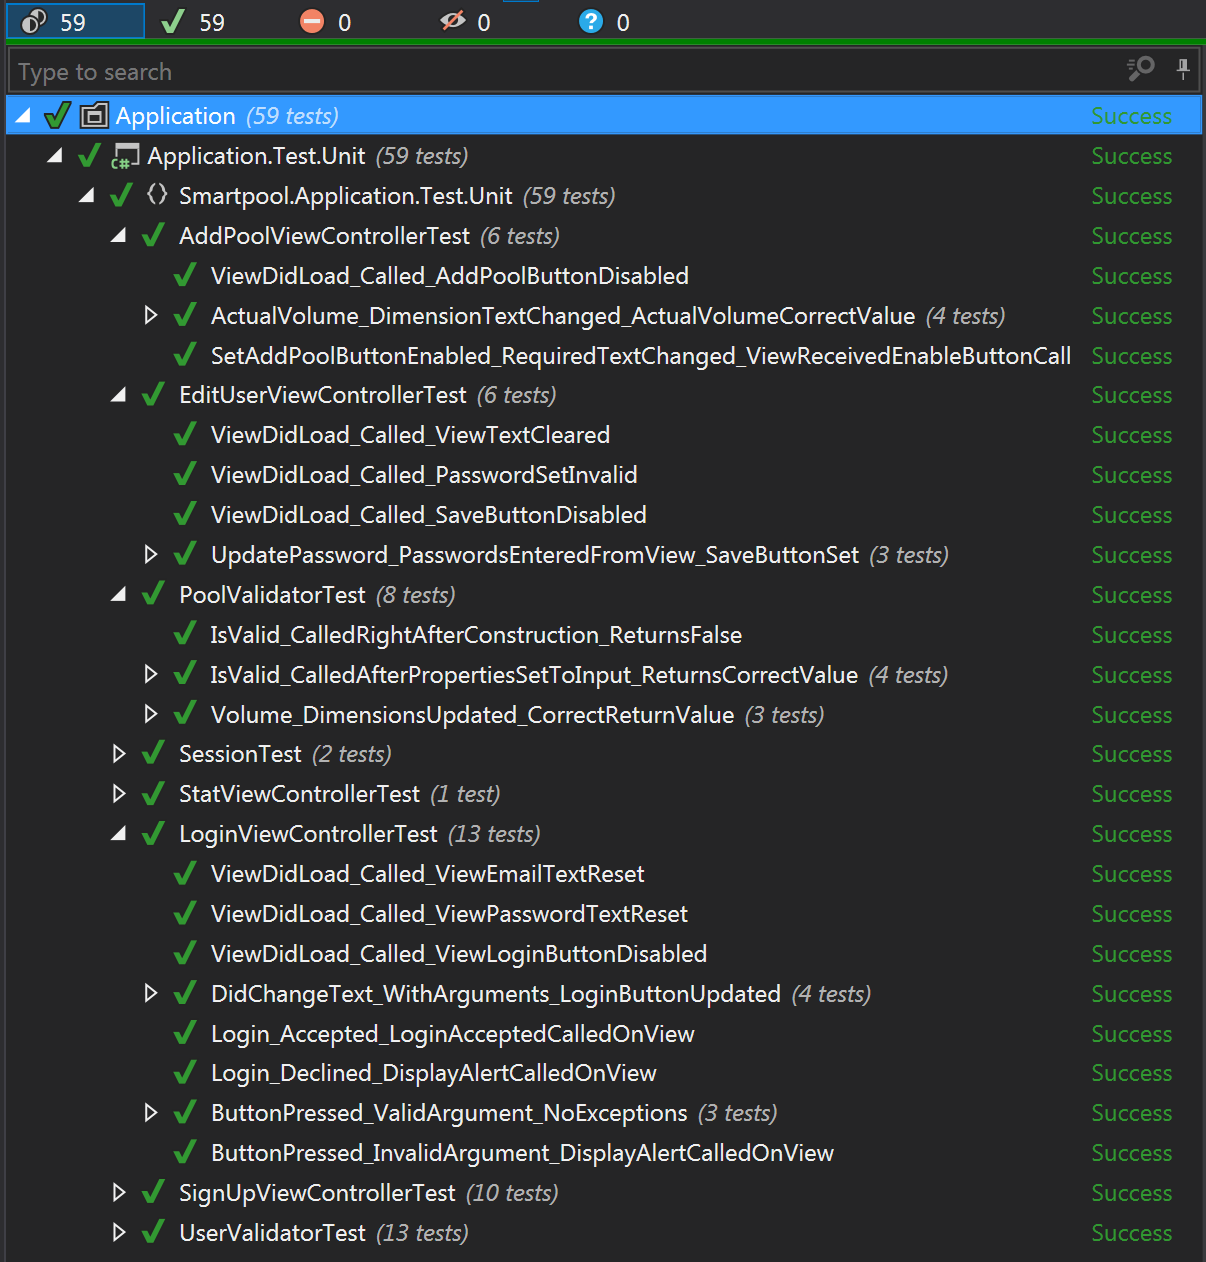
\includegraphics[width=0.9\linewidth]{figs/test/apptest}
\caption{Test af applikationslaget.}
\label{fig:apptest}
\end{figure}

I forbindelse med unit-test kører vi code coverage målinger, for at få en idé om, hvilke dele af klasserne der er testet. På figur~\ref{fig:appcoverage} ses code coverage resultatet for test-suiten. Som det fremgår af code-coverage analysen, er GUI applikationen Win (og de andre GUI applikationer), ikke testet med NUnit, og har derfor ingen code coverage.

% BILLEDE AF COVERAGE KØRT
\begin{figure}
\centering
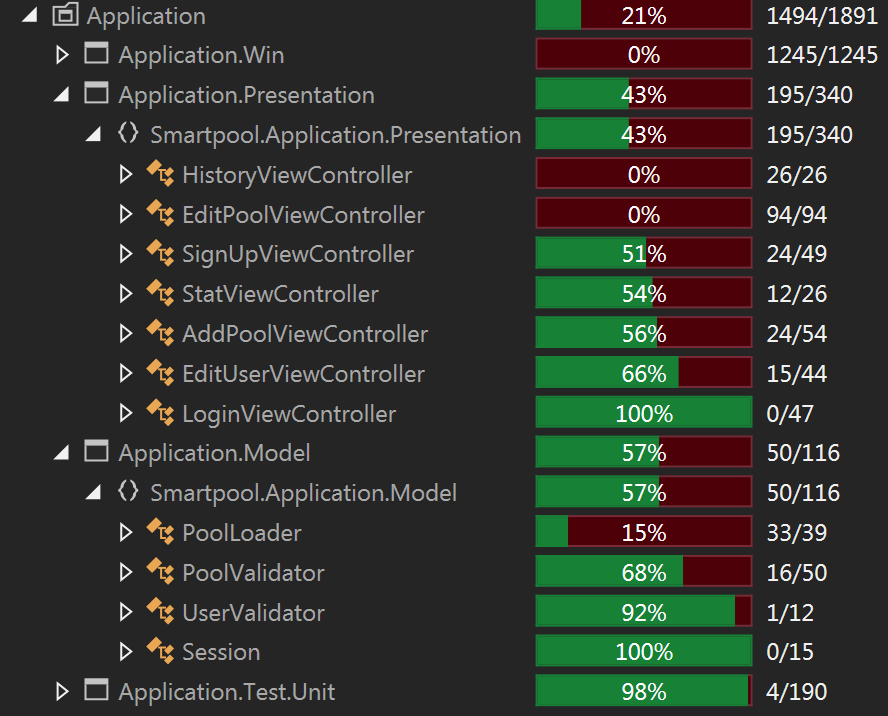
\includegraphics[width=0.9\linewidth]{figs/test/appcoverage}
\caption{Code coverage for applikationslaget.}
\label{fig:appcoverage}
\end{figure}

\subsection{Testbeskrivelse}
% hvordan div. test er valgt og hvad I specielt var opmærksom på under udviklign af test. 
% hvad var let/svært at teste etc.
Modelklasserne i applikationslaget har få afhængigheder, og kan derfor testes uden brug af fakes. Modelklasserne testes individuelt, og den ene klasse (PoolLoader) der benytter sig af en IClientMessenger, opsættes med en fake IClientMessenger. Presenter-klasserne testes også individuelt, og deres dependency til et IView og en IClientMessenger fakes med NSubstitute. I Presenter-klasserne testes forskellige metodekald, samt interaktionen med fake view’s (mocks). Model-klasserne i Smartpool.Application.Model implementerer ikke interfaces. Dette var en ulempe, der gjorde test af presenter-klasser, sværere end de burde have været. Dette er også grundet til, at code-coverage procenten i præsentationslaget er lav. Grundet tidsbegrænsning nåede denne problemstilling ikke at blive rettet i projektforløbet, men opmærsomhed har været rettet på det.

Da både presenter-klasser og model er testet med førnævnte test-suite, elimineres en stor del af de logiske fejl som kan opstå i GUI-projekterne. View-implementeringen indeholder udelukkende logik, vedrørende view’ets udseende og hvordan data præsenteres.